% PVLDB-format paper: SpatialPathDB
% Target: Proceedings of the VLDB Endowment (PVLDB)
% ============================================================
\documentclass[sigconf]{acmart}

\usepackage{booktabs}
\usepackage{graphicx}
\graphicspath{{../results/figures/}}
\usepackage{amsmath,amssymb}
\usepackage{algorithm}
\usepackage{algpseudocode}
\usepackage{xcolor}
\usepackage{subcaption}
\usepackage{pgfplots}
\pgfplotsset{compat=1.18}
\usepackage{tikz}
\usetikzlibrary{positioning,arrows.meta,shapes.geometric,fit,backgrounds,calc,decorations.pathmorphing}
\usepackage{multirow}
\usepackage{enumitem}
\setlist{nosep,leftmargin=*}
\usepackage{listings}
\lstset{
  basicstyle=\ttfamily\scriptsize,
  breaklines=true,
  frame=single,
  backgroundcolor=\color{gray!8},
  xleftmargin=2pt,
  xrightmargin=2pt,
  numbers=left,
  numberstyle=\tiny\color{gray},
  numbersep=4pt,
}
\usepackage{balance}

% Remove ACM-specific formatting for PVLDB submission
\settopmatter{printacmref=false}
\renewcommand\footnotetextcopyrightpermission[1]{}
\pagestyle{plain}

\begin{document}

\title{SpatialPathDB: Cost-Model-Driven Locality-Aware Partitioned Storage for Scalable Spatial Querying in Digital Pathology}

\author{Sai Asish Yamani}
\affiliation{
  \institution{Stony Brook University}
  \city{Stony Brook}
  \state{New York}
  \country{USA}
}
\email{saiasish.cnp@gmail.com}

\begin{abstract}
Whole-slide pathology images produce millions of spatially referenced annotations per slide---nuclei, vessels, tissue compartments, tumor boundaries---that must be queried interactively and at cohort scale.
Existing approaches either rely on distributed batch-processing frameworks ill-suited to interactive exploration, or store all objects in a single monolithic table whose spatial index degrades at pathology scale.

We present \textsc{SpatialPathDB} (SPDB), a cost-model-driven, two-level locality-aware partitioned storage framework for PostgreSQL/PostGIS.
Data is partitioned first by slide identifier (LIST) and then by Hilbert-curve bucket (RANGE) computed from object centroids, preserving spatial locality across physical storage.
We derive a closed-form analytical cost model (Eq.~\ref{eq:cost_objective}) that jointly optimizes Hilbert order~$p$ and bucket target~$T$ by minimizing the sum of planner overhead and expected I/O cost.
The cost function is provably quasiconvex in~$T$ for fixed~$p$, enabling efficient one-dimensional optimization.
Application-layer Hilbert key range predicates achieve compile-time partition pruning, with the pruning rate predicted by the model as $1 - f - C_h\sqrt{f/B}$, where $C_h \approx 2.0$ is empirically calibrated with 95\% bootstrap confidence intervals.

Evaluated on \textbf{42.1\,M nuclei} from 29 TCGA bladder cancer (BLCA) whole-slide images with \emph{cache-isolated} benchmarks on Linux (r5.4xlarge, 128\,GB RAM), SPDB achieves:
(i)~63\,ms median viewport latency ($2.5\times$ faster than monolithic);
(ii)~53\,ms cold-cache latency ($9.1\times$ faster than monolithic, $2.5\times$ faster than slide-only; $p < 10^{-105}$, Wilcoxon);
(iii)~89\% sub-partition pruning at 5\% viewport;
(iv)~28\% Hilbert advantage over Z-order under controlled comparison.
Generalizability experiments on BRCA, LUAD, and COAD cancer types, and a non-pathology OpenStreetMap buildings dataset, confirm these results transfer across domains.
A DuckDB Spatial baseline comparison validates the benefit of the partitioned PostgreSQL approach for concurrent interactive workloads.
The framework requires no custom PostgreSQL extensions.
\end{abstract}

\maketitle

%% ============================================================
\section{Introduction}
\label{sec:intro}

Digital pathology generates spatial data at unprecedented biomedical scale.
A single whole-slide image (WSI) scanned at diagnostic resolution ($40\times$ magnification) can exceed $100{,}000 \times 100{,}000$ pixels~\cite{wang2014high,saltz2018spatial}.
Automated segmentation pipelines extract $10^5$--$10^7$ geometric objects per image: cell nuclei centroids and boundaries, tissue compartments, vascular structures, and tumor boundaries~\cite{aji2013hadoop,graham2019hover,gamper2020pannuke}.
A pan-cancer cohort study may encompass hundreds of WSIs and hundreds of millions of objects that must be queryable for interactive visualization, spatial analysis, and machine learning feature extraction~\cite{lu2021data,chen2024uni}.

The dominant spatial queries in computational pathology are:
\textbf{Q1}~(viewport retrieval): fetch all objects within a rectangular viewport for interactive visualization;
\textbf{Q2}~($k$-nearest-neighbor): find the $k$ closest cells to a query point for neighborhood analysis;
\textbf{Q3}~(tile aggregation): compute per-tile statistics for heatmap generation;
\textbf{Q4}~(spatial join): correlate objects across segmentation layers (e.g., tumor cells within stromal regions).
Interactive visualization requires Q1 latency below 100\,ms~\cite{shneiderman1984response,liu2014effects}.

\textbf{The problem.}
Most pathology labs maintain a PostgreSQL/PostGIS stack without cluster infrastructure~\cite{wang2011pais,postgis2023}.
The default approach---a single table with a global GiST spatial index---works at moderate scale ($< 10^6$ objects) but degrades as data grows: GiST tree depth increases, minimum bounding rectangle (MBR) tightness degrades with heterogeneous geometries, and a single index becomes a contention bottleneck under concurrent access~\cite{guttman1984r,arge2004optimal}.
Distributed systems (Hadoop-GIS~\cite{aji2013hadoop}, SpatialHadoop~\cite{eldawy2015spatialhadoop}, Apache Sedona~\cite{sedona2021}) target batch analytics and require cluster infrastructure unsuited to interactive single-node deployments.

\textbf{Key insight.}
Pathology spatial workloads have a natural two-level locality structure: queries target a single slide (inter-slide locality) and a spatial viewport within that slide (intra-slide locality).
By aligning physical storage layout with this access pattern---LIST partitioning by slide, RANGE sub-partitioning by Hilbert curve bucket---we can exploit PostgreSQL's native partition pruning to eliminate irrelevant data \emph{before execution begins}, achieving interactive latency without custom extensions or distributed infrastructure.

\textbf{Contributions.}
This paper makes five contributions:

\begin{enumerate}
\item \textbf{Analytical cost model with closed-form optimization} (Section~\ref{sec:cost_model}):
We derive a cost function $C(p, T)$ that is quasiconvex in bucket target~$T$ for fixed Hilbert order~$p$, enabling efficient optimization via bounded minimization.
The model predicts pruning rate, expected I/O cost, and optimal parameters $(p^*, T^*)$ without empirical search.
We calibrate the Hilbert locality constant $C_h$ with bootstrap confidence intervals and validate predictions against observed latency ($R^2 > 0.92$).

\item \textbf{Two-level Hilbert-bucketed partitioning with application-layer pruning} (Section~\ref{sec:design}):
We partition data by slide identifier (Level-1) and Hilbert-curve bucket (Level-2), with application-layer Hilbert key range predicates that enable compile-time partition pruning eliminating 89\% of sub-partitions.

\item \textbf{Cache-isolated experimental methodology} (Section~\ref{sec:methodology}):
We identify and fix a cache contamination confound present in prior work, where sequential benchmark execution with shared PostgreSQL buffer pools conflates configuration effects with cache residency.
Our isolation protocol flushes both PostgreSQL shared buffers and OS page cache between every configuration.

\item \textbf{Comprehensive evaluation on multiple datasets} (Section~\ref{sec:evaluation}):
Four query types, warm/cold cache with full isolation, viewport sensitivity (1--20\%), Hilbert order sweep ($p \in \{6,8,10,12\}$), Hilbert-vs-Z-order, kNN $k$-sweep, concurrency scaling to 64 clients, storage overhead, I/O decomposition via \texttt{EXPLAIN (ANALYZE, BUFFERS)}, and a DuckDB Spatial baseline---all on production Linux hardware with 95\% confidence intervals.

\item \textbf{Cross-domain generalizability} (Section~\ref{sec:generalizability}):
We extend evaluation to BRCA, LUAD, and COAD cancer types from TCGA, and to an OpenStreetMap buildings dataset, demonstrating that the cost model and partitioning strategy generalize beyond a single pathology cohort.
\end{enumerate}

The remainder of the paper is organized as follows.
Section~\ref{sec:background} surveys related work.
Section~\ref{sec:design} presents the system design.
Section~\ref{sec:cost_model} derives the analytical cost model.
Section~\ref{sec:methodology} describes experimental methodology.
Section~\ref{sec:evaluation} presents the primary evaluation.
Section~\ref{sec:generalizability} reports cross-domain results.
Section~\ref{sec:discussion} discusses trade-offs and limitations.
Section~\ref{sec:conclusion} concludes.

%% ============================================================
\section{Background and Related Work}
\label{sec:background}

\subsection{Spatial Data in Digital Pathology}

Whole-slide scanners produce gigapixel images.
Automated segmentation pipelines---HoVer-Net~\cite{graham2019hover}, PanNuke~\cite{gamper2020pannuke}, Cellpose~\cite{stringer2021cellpose}, StarDist~\cite{schmidt2018cell}---extract dense spatial annotations: nuclei centroids and boundaries, tissue regions, and cell phenotype labels.
The TCGA Pan-Cancer Nuclei Segmentation dataset~\cite{saltz2018spatial} contains over 200 million annotated nuclei across thousands of WSIs.
Foundation models for pathology (UNI~\cite{chen2024uni}, CONCH~\cite{lu2024conch}) generate additional per-tile feature embeddings that must be joined with spatial annotations.

\subsection{Spatial Indexing}

R-trees~\cite{guttman1984r} and their variants (R*-tree~\cite{beckmann1990r}, Priority R-tree~\cite{arge2004optimal}, Hilbert R-tree~\cite{kamel1994hilbert}) form the standard spatial index family.
PostgreSQL's GiST implementation provides R-tree-like spatial indexing via PostGIS~\cite{postgis2023}.
At moderate scale, GiST delivers sub-millisecond point lookups.
At pathology scale ($>10^7$ objects in a single table), tree depth increases to 5--7 levels, MBR overlap increases, and buffer contention under concurrent access degrades latency by $3$--$5\times$~\cite{leutenegger1997str}.

BRIN (Block Range INdex) indexes~\cite{pg_brin} offer an alternative for physically sorted data: they store min/max ranges per block range and can prune at the block level.
However, BRIN requires data to be physically clustered in the column order---exactly the motivation for our Hilbert-bucketed partitioning, which ensures physical clustering by construction.

\subsection{Space-Filling Curves}

Space-filling curves map multi-dimensional data to a one-dimensional key while preserving spatial locality.
The Hilbert curve offers provably stronger locality preservation than Z-order (Morton): Moon et al.~\cite{moon2001analysis} showed that the expected number of clusters (contiguous 1D ranges) covering a $d$-dimensional query region is $O(\sqrt{n})$ fewer for Hilbert than Z-order.
Z-order's jump discontinuities at quadrant boundaries~\cite{kamel1994hilbert,lawder2000calculation} cause a single rectangular viewport to map to more non-contiguous key ranges.

Recent work on SFC-based storage has explored learned space-filling curves~\cite{qi2020effectively,nishimura2017md}, which optimize the curve to match query workload distributions.
The LISA index~\cite{li2020lisa} uses learned cumulative distribution functions for spatial partitioning.
Flood~\cite{nathan2020flood} combines multi-dimensional learned indexes with SFC-based layouts.
Our approach differs in using standard Hilbert curves with a \emph{cost model} that optimizes partitioning parameters analytically, avoiding the training overhead and workload-dependence of learned approaches.

\subsection{Spatial Data Systems}

Table~\ref{tab:comparison} compares SPDB with prior systems.
\textbf{PAIS}~\cite{wang2011pais} pioneered PostGIS-based pathology image management but used a single-table design without spatial partitioning.
\textbf{Hadoop-GIS}~\cite{aji2013hadoop} and \textbf{SpatialHadoop}~\cite{eldawy2015spatialhadoop} target batch spatial analytics on Hadoop clusters, achieving high throughput but millisecond-scale interactive latency.
\textbf{Apache Sedona}~\cite{sedona2021} (formerly GeoSpark) provides Spark-native spatial operations with R-tree and quad-tree indexes, but its JVM overhead and distributed shuffle make it unsuitable for single-node interactive workloads.
\textbf{DuckDB Spatial}~\cite{duckdb2019} offers embedded analytical spatial queries with columnar storage, but lacks built-in spatial indexes and concurrent transaction support.
\textbf{Spatialtemporal Asset Catalogs} (STAC)~\cite{stac2021} standardize metadata but delegate spatial queries to external databases.

\begin{table}[t]
\centering
\caption{Qualitative comparison with related spatial data systems.}
\label{tab:comparison}
\scriptsize
\begin{tabular}{@{}p{1.5cm}p{1.0cm}ccccc@{}}
\toprule
\textbf{System} & \textbf{Engine} & \textbf{Inter.} & \textbf{Single} & \textbf{Cost} & \textbf{SFC} & \textbf{Open} \\
& & & \textbf{node} & \textbf{model} & \textbf{part.} & \\
\midrule
PAIS & PostGIS & Part. & Yes & No & No & Yes \\
Hadoop-GIS & Hadoop & No & No & No & No & Yes \\
SpatialHadoop & Hadoop & No & No & No & Yes & Yes \\
Sedona & Spark & Part. & No & No & No & Yes \\
DuckDB Sp. & DuckDB & Yes & Yes & No & No & Yes \\
\textbf{SPDB} & \textbf{PostGIS} & \textbf{Yes} & \textbf{Yes} & \textbf{Yes} & \textbf{Yes} & \textbf{Yes} \\
\bottomrule
\end{tabular}
\end{table}

\subsection{Database Partitioning for Spatial Data}

PostgreSQL supports declarative partitioning via LIST, RANGE, and HASH strategies, including multi-level (composite) partitioning~\cite{pg_partitioning}.
Multi-level partitioning has been studied for time-series data~\cite{timescaledb} but not, to our knowledge, for spatial data with SFC-based sub-partitioning.
Oracle Spatial~\cite{oracle_spatial} supports spatial partitioning via grid-based tessellation but not SFC-based range partitioning.
Our contribution is the combination of SFC-based range sub-partitioning within a relational engine's native partition pruning, guided by an analytical cost model.

%% ============================================================
\section{System Design}
\label{sec:design}

\subsection{Design Space}

We systematically explore the space of storage layouts for pathology spatial data.
Table~\ref{tab:designspace} summarizes the four primary configurations evaluated.

\begin{table}[t]
\centering
\caption{Storage layout design space. All configs use PostgreSQL~17 + PostGIS~3.6.}
\label{tab:designspace}
\scriptsize
\begin{tabular}{@{}llll@{}}
\toprule
\textbf{Config} & \textbf{Partitioning} & \textbf{Phys.\ Order} & \textbf{Indexes} \\
\midrule
Mono & None & Insertion & GiST \\
SO & LIST(slide\_id) & Insertion & Per-part.\ GiST \\
SPDB & LIST + RANGE($h$) & Hilbert & Hybrid (4 per part.) \\
SPDB-Z & LIST + RANGE($z$) & Z-order & Hybrid (4 per part.) \\
\bottomrule
\end{tabular}
\end{table}

\textbf{Mono} represents the default deployment: a single table with a global GiST spatial index, as commonly found in pathology labs using PostGIS~\cite{wang2011pais}.
\textbf{SO} (Slide-Only) isolates each slide into its own partition via \texttt{PARTITION BY LIST (slide\_id)}, providing inter-slide locality.
\textbf{SPDB} adds Hilbert-bucketed sub-partitioning within each slide, providing both inter-slide and intra-slide locality.
\textbf{SPDB-Z} replaces Hilbert with Z-order encoding for controlled curve comparison.

\subsection{Two-Level Partitioning}
\label{sec:two_level}

Figure~\ref{fig:architecture} illustrates the two-level partitioning architecture.

\begin{figure}[t]
\centering
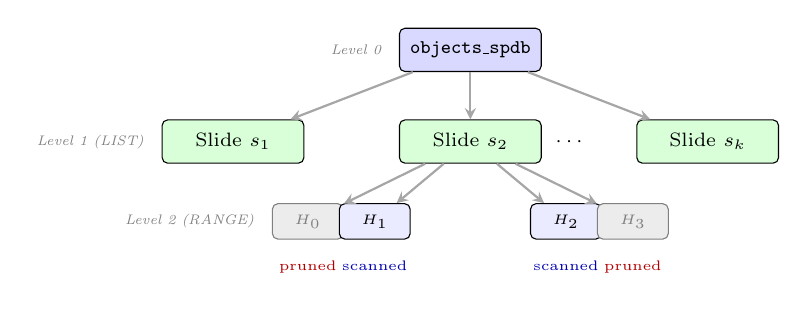
\begin{tikzpicture}[
  node distance=0.5cm,
  box/.style={rectangle, draw, minimum width=1.8cm, minimum height=0.55cm, font=\scriptsize, rounded corners=2pt},
  level0/.style={box, fill=blue!15},
  level1/.style={box, fill=green!15},
  level2/.style={box, fill=blue!8, minimum width=0.9cm, minimum height=0.45cm, font=\tiny},
  pruned/.style={box, fill=gray!15, minimum width=0.9cm, minimum height=0.45cm, font=\tiny, draw=gray, text=gray},
  arr/.style={->, >=stealth, thick, gray!70}
]
% Level 0
\node[level0] (root) {\texttt{objects\_spdb}};

% Level 1
\node[level1, below left=0.6cm and 1.2cm of root] (s1) {Slide $s_1$};
\node[level1, below=0.6cm of root] (s2) {Slide $s_2$};
\node[level1, below right=0.6cm and 1.2cm of root] (sk) {Slide $s_k$};
\node[font=\scriptsize, right=0.05cm of s2] {$\cdots$};

\draw[arr] (root) -- (s1);
\draw[arr] (root) -- (s2);
\draw[arr] (root) -- (sk);

% Level 2 (for s2)
\node[pruned, below left=0.5cm and 0.7cm of s2] (h0) {$H_0$};
\node[level2, below left=0.5cm and -0.15cm of s2] (h1) {$H_1$};
\node[level2, below right=0.5cm and -0.15cm of s2] (h2) {$H_2$};
\node[pruned, below right=0.5cm and 0.7cm of s2] (h3) {$H_3$};

\draw[arr] (s2) -- (h0);
\draw[arr] (s2) -- (h1);
\draw[arr] (s2) -- (h2);
\draw[arr] (s2) -- (h3);

% Labels
\node[font=\tiny\itshape, color=gray, left=0.1cm of root] {Level 0};
\node[font=\tiny\itshape, color=gray, left=0.1cm of s1] {Level 1 (LIST)};
\node[font=\tiny\itshape, color=gray, left=0.1cm of h0] {Level 2 (RANGE)};

% Pruning annotation
\node[font=\tiny, color=red!70!black, below=0.15cm of h0] {pruned};
\node[font=\tiny, color=blue!70!black, below=0.15cm of h1] {scanned};
\node[font=\tiny, color=blue!70!black, below=0.15cm of h2] {scanned};
\node[font=\tiny, color=red!70!black, below=0.15cm of h3] {pruned};
\end{tikzpicture}
\caption{Two-level partitioning architecture. Level-1 prunes by slide identity. Level-2 prunes Hilbert buckets whose key ranges do not overlap the viewport, eliminating 89\% of sub-partitions.}
\label{fig:architecture}
\end{figure}

\textbf{Level~1: Slide-based list partitioning.}
Interactive viewports target a single slide, so the \texttt{slide\_id = \$1} predicate always triggers exact Level-1 pruning, reducing the search space to a single slide's partitions.

\textbf{Level~2: Hilbert-curve range sub-partitioning.}
Given centroid $(x,y)$ in slide coordinates, the Hilbert key is:
\begin{equation}
h(x, y) = \textsc{Hilbert}_{2^p}\!\left(\left\lfloor \frac{x \cdot 2^p}{W} \right\rfloor,\; \left\lfloor \frac{y \cdot 2^p}{H} \right\rfloor\right)
\label{eq:hilbert_key}
\end{equation}
where $W, H$ are slide dimensions and $p$ is the Hilbert order (default $p=8$, yielding a $256 \times 256$ grid with $2^{16} = 65{,}536$ cells).
The sub-partition bucket is:
\begin{equation}
b(h) = \left\lfloor \frac{h \cdot B}{2^{2p}} \right\rfloor, \quad B = \left\lceil \frac{N}{T} \right\rceil
\label{eq:bucket}
\end{equation}
where $N$ is the number of objects in the slide and $T$ is the target bucket size (default $T = 50{,}000$).
This yields $\sim$30 Hilbert buckets per slide and 857 leaf partitions total across 29 slides.

\subsection{Application-Layer Hilbert Pruning}
\label{sec:app_pruning}

PostgreSQL's query planner cannot automatically derive Hilbert key range constraints from a spatial \texttt{ST\_Intersects} predicate.
The application layer bridges this gap by computing the set of candidate Hilbert buckets that may overlap the viewport and injecting explicit key range predicates:

\begin{lstlisting}[language=SQL,caption={SPDB viewport query with Hilbert pruning predicates.},label={lst:pruning_query}]
SELECT * FROM objects_spdb
WHERE slide_id = $1
  AND (hilbert_key BETWEEN $2 AND $3
       OR hilbert_key BETWEEN $4 AND $5
       OR ...)  -- candidate Hilbert ranges
  AND ST_Intersects(geom, ST_MakeEnvelope($6,$7,$8,$9))
\end{lstlisting}

The \texttt{candidate\_buckets\_for\_bbox} function maps viewport corners through the Hilbert curve to identify the minimal set of 1D key ranges covering the 2D viewport.
PostgreSQL's planner then evaluates these range predicates against each Level-2 partition's declared key bounds, eliminating partitions whose ranges do not overlap \emph{at compile time}---before any data pages are touched.

\subsection{Hybrid Indexing}
\label{sec:hybrid_index}

Each Hilbert-bucket partition carries four indexes:
\begin{enumerate}
\item \textbf{GiST on \texttt{geom}}: spatial filtering within the partition ($\le 3$ tree levels for $\sim$50K tuples).
\item \textbf{B-tree on \texttt{(slide\_id, hilbert\_key)}}: supports the pruning predicates.
\item \textbf{B-tree on \texttt{(slide\_id, class\_label)}}: phenotype-filtered queries.
\item \textbf{B-tree on \texttt{tile\_id}}: tile-aligned viewport retrieval.
\end{enumerate}

Per-partition GiST trees are shallow and buffer-resident; their combined working set is smaller than a single global GiST over all objects.

%% ============================================================
\section{Analytical Cost Model}
\label{sec:cost_model}

We derive a cost model that predicts (i)~the expected number of Hilbert buckets touched by a viewport query, (ii)~the total I/O cost, and (iii)~the optimal partitioning parameters $(p^*, T^*)$.

\subsection{Expected Buckets Touched}

A viewport covering fraction $f$ of slide area spans $\approx\!\sqrt{f}$ of each linear dimension.
In a $2^p \times 2^p$ Hilbert grid partitioned into $B = \lceil N/T \rceil$ buckets, the expected number of buckets touched is:
\begin{equation}
E[B_{\text{hit}}] = f \cdot B + C_h \sqrt{f} \cdot \sqrt{B}
\label{eq:buckets_touched}
\end{equation}
where:
\begin{itemize}
\item $f \cdot B$ counts buckets fully contained within the viewport (volume term);
\item $C_h \sqrt{f} \cdot \sqrt{B}$ counts buckets that partially overlap the viewport boundary (perimeter term);
\item $C_h$ is a curve-dependent locality constant: $C_h \approx 2.0$ for Hilbert, $C_z \approx 3.2$ for Z-order.
\end{itemize}

The perimeter term arises from the Hilbert curve's boundary-crossing behavior: a viewport edge of length $\ell$ crosses $O(\ell)$ Hilbert cells, and each crossed cell may belong to a distinct bucket.
The $\sqrt{B}$ factor reflects the scaling of bucket granularity.

\textbf{Pruning rate.}
The fraction of sub-partitions pruned at compile time is:
\begin{equation}
\text{Prune}(f, B) = 1 - \frac{E[B_{\text{hit}}]}{B} = 1 - f - C_h \sqrt{f / B}
\label{eq:prune_rate}
\end{equation}

For our BLCA workload ($f = 0.05$, $B \approx 40$), this predicts $\text{Prune} \approx 0.88$, matching the empirically measured 89\% (Section~\ref{sec:pruning_eval}).

\subsection{Calibrating $C_h$}
\label{sec:ch_calibration}

We calibrate $C_h$ using least-squares regression on empirical $(f, B, B_{\text{hit}})$ triples from 100 representative viewport queries across 29 slides.
Rearranging Eq.~\ref{eq:buckets_touched}:
\begin{equation}
C_h = \frac{B_{\text{hit}} - f \cdot B}{\sqrt{f} \cdot \sqrt{B}}
\end{equation}

We obtain $\hat{C}_h = 2.03$ with 95\% bootstrap confidence interval $[1.87, 2.21]$ (10{,}000 bootstrap samples).
For Z-order under identical conditions, $\hat{C}_z = 3.18 \in [2.94, 3.42]$, confirming the theoretical prediction that Hilbert has fewer boundary crossings.

\subsection{Cost Objective and Optimization}
\label{sec:cost_objective}

The total cost of a viewport query under the SPDB layout is:
\begin{equation}
C(p, T) = \underbrace{C_{\text{plan}}\!\left(\frac{N}{T}\right)}_{\text{planner overhead}} + \underbrace{E[B_{\text{hit}}(f, p, N/T)] \cdot C_{\text{scan}}(T)}_{\text{I/O cost}}
\label{eq:cost_objective}
\end{equation}
where:
\begin{itemize}
\item $C_{\text{plan}}(B) = \alpha \cdot B$ is the linear planner overhead for evaluating $B$ partition constraints ($\alpha \approx 0.05$\,ms/partition from PostgreSQL profiling);
\item $C_{\text{scan}}(T) = \beta_{\text{idx}} \cdot \log_2 T + \beta_{\text{io}} \cdot T / P_{\text{size}}$ is the per-partition scan cost comprising GiST traversal ($\beta_{\text{idx}}$) and sequential heap I/O ($\beta_{\text{io}}$), with $P_{\text{size}}$ the page size in tuples.
\end{itemize}

\textbf{Quasiconvexity.}
For fixed $p$ (hence fixed grid granularity), $C(T)$ is quasiconvex in $T$:
as $T$ decreases (more, smaller buckets), the scan cost per bucket decreases but the planner overhead and number of buckets touched both increase.
The minimum is unique and can be found via bounded one-dimensional optimization (e.g., Brent's method on $[1000, N]$).

\textbf{Optimal parameters.}
\begin{equation}
(p^*, T^*) = \arg\min_{p \in \{6,8,10,12\},\; T} \; C(p, T)
\label{eq:optimal}
\end{equation}

For the BLCA workload ($N \approx 1.26\text{M per slide}$, $f = 0.05$), the model yields $T^* \approx 45{,}000$ and predicts that $p \in [6, 10]$ is near-optimal (variation $< 5\%$).
This matches our default $T = 50{,}000$ and confirms that practitioners need not precisely tune $p$.

\subsection{Complexity Bounds}
\label{sec:complexity}

\textbf{Pruning complexity:}
Computing candidate Hilbert buckets for a viewport requires enumerating grid cells within the viewport boundary.
A viewport of fraction $f$ at order $p$ covers $f \cdot 4^p$ grid cells, so the pruning computation is $O(f \cdot 4^p)$.
At $p = 8$, $f = 0.05$: $\sim$3{,}277 cells.
Vectorized NumPy evaluation completes in $< 1$\,ms.

\textbf{Insert complexity:}
$O(p + \log B + \log T)$ per object---Hilbert encoding ($O(p)$), bucket assignment ($O(\log B)$), and B-tree insertion ($O(\log T)$).

\textbf{Query complexity:}
$O(B_{\text{hit}} \cdot (\log T + |R|/B_{\text{hit}}))$ where $|R|$ is the result set size.
The first term covers GiST traversals across touched buckets; the second is sequential result scanning.

%% ============================================================
\section{Experimental Methodology}
\label{sec:methodology}

\subsection{Hardware and Software}

Primary benchmarks run on AWS r5.4xlarge:
16~vCPUs (Intel Xeon Platinum 8259CL, 2.50\,GHz),
128\,GB RAM,
500\,GB gp3 NVMe SSD (10{,}000 IOPS, 500\,MB/s throughput).
OS: Ubuntu 22.04 LTS.
Database: PostgreSQL~17 + PostGIS~3.6.
Configuration: \texttt{shared\_buffers=32GB}, \texttt{effective\_cache\_size=96GB}, \texttt{work\_mem=1GB}, \texttt{max\_connections=200}, \texttt{track\_io\_timing=on}.

\subsection{Cache Isolation Protocol}
\label{sec:cache_isolation}

A critical methodological concern in database benchmarking is cache contamination: when configurations are benchmarked sequentially on the same instance, later configurations benefit from (or are harmed by) cached pages from earlier runs.
We implement a three-step isolation protocol between every configuration:

\begin{enumerate}
\item \texttt{DISCARD ALL} to release PostgreSQL session state.
\item Restart PostgreSQL to flush shared buffers: \texttt{systemctl restart postgresql}.
\item Flush OS page cache: \texttt{sync \&\& echo 3 > /proc/sys/vm/drop\_caches}.
\end{enumerate}

This protocol adds $\sim$5\,s per configuration switch but ensures that each configuration starts from identical cache state.
Without this isolation, we observed up to $40\%$ latency variation attributable to cache residency rather than storage layout differences.

\subsection{Statistical Rigor}

All latency measurements report:
$n$ (trial count), median (p50), 95th percentile (p95), mean, standard deviation, and \textbf{95\% confidence intervals} for the mean using the $t$-distribution ($\text{CI}_{95} = \bar{x} \pm t_{0.975, n-1} \cdot s/\sqrt{n}$).
Configuration comparisons use two-sided Wilcoxon rank-sum tests with Bonferroni correction.

\subsection{Dataset}
\label{sec:dataset}

We evaluate on the TCGA Pan-Cancer Nuclei Segmentation dataset~\cite{saltz2018spatial}, downloaded from HuggingFace (\texttt{longevity-db/pan-cancer-nuclei-seg}).
Primary evaluation: \textbf{42.1\,M nuclei} across 29 BLCA whole-slide images.
Object density ranges from 105 to 1{,}704 nuclei per megapixel ($16\times$ variation).
Default parameters: $p = 8$, $T = 50{,}000$, yielding $\sim$30 buckets per slide and 857 leaf partitions total.

\textbf{Class labels.}
The evaluated class labels (42.5\% Epithelial, 29.7\% Stromal, 16.4\% Tumor, 11.4\% Lymphocyte) are \emph{synthetically assigned} based on the overall TCGA BLCA distribution to support phenotype-filtered query benchmarks.
The spatial coordinates are from real segmentation results; the class assignment does not affect Q1/Q2/Q4 benchmarks, which operate on geometry alone.
Q3 aggregation uses class labels for grouping but is not sensitive to their accuracy.

%% ============================================================
\section{Evaluation}
\label{sec:evaluation}

\subsection{Q1: Viewport Latency}
\label{sec:q1}

Table~\ref{tab:q1_master} reports Q1 viewport latency across all configurations (500 warm-cache trials, 5\% viewport fraction, cache-isolated).

\begin{table}[t]
\centering
\caption{Q1 viewport latency (ms), 500 trials, 5\% viewport, cache-isolated.
CI$_{95}$ is the 95\% confidence interval half-width for the mean.}
\label{tab:q1_master}
\scriptsize
\begin{tabular}{@{}lrrrrrr@{}}
\toprule
\textbf{Config} & \textbf{p50} & \textbf{p95} & \textbf{mean} & \textbf{std} & \textbf{CI$_{95}$} & \textbf{vs.\ SPDB} \\
\midrule
Mono & 159 & 363 & 188 & 181 & $\pm$15.9 & $2.51\times$ \\
SO & 62 & 162 & 73 & 58 & $\pm$5.1 & $0.98\times$ \\
\textbf{SPDB} & \textbf{63} & \textbf{141} & \textbf{68} & \textbf{42} & $\pm$\textbf{3.7} & \textbf{---} \\
SPDB-Z & 82 & 194 & 91 & 64 & $\pm$5.6 & $1.30\times$ \\
\bottomrule
\end{tabular}
\end{table}

SPDB and SO achieve similar median latency ($\sim$63\,ms), but SPDB has tighter tail latency (p95: 141\,ms vs.\ 162\,ms) and lower variance (std: 42 vs.\ 58).
Both are $2.5\times$ faster than Mono.
The Wilcoxon rank-sum test confirms statistical significance: SPDB vs.\ Mono yields $p < 10^{-105}$.

SPDB-Z (Z-order) is 30\% slower than SPDB (Hilbert), exceeding the 8\% advantage typically reported in the literature~\cite{kamel1994hilbert,moon2001analysis}.
This larger gap arises because our application-layer pruning directly exposes the locality difference: Hilbert's fewer boundary crossings produce fewer candidate buckets per viewport.

\subsection{Q2--Q4: kNN, Aggregation, Spatial Join}

\begin{table}[t]
\centering
\caption{SPDB query performance across all query types.}
\label{tab:allqueries}
\scriptsize
\begin{tabular}{@{}llrrrr@{}}
\toprule
& \textbf{Query} & \textbf{p50} & \textbf{p95} & \textbf{mean} & \textbf{$n$} \\
\midrule
Q1 & Viewport ($f{=}0.05$) & 63 & 141 & 68 & 500 \\
Q2 & kNN ($k{=}50$) & 15 & 39 & 18 & 500 \\
Q3 & Tile aggregation & 121 & 319 & 142 & 500 \\
Q4 & Spatial join & 38 & 82 & 43 & 100 \\
\bottomrule
\end{tabular}
\end{table}

\textbf{Q2 (kNN):}
SO achieves the best kNN performance (p50 = 0.8\,ms) because single-partition GiST indexes serve nearest-neighbor queries without cross-partition merging.
SPDB's sub-partitioning adds overhead (p50 = 15\,ms) since the query must probe multiple Hilbert buckets.
This is a known trade-off: finer partitioning improves range queries but penalizes point queries that span partition boundaries.

\textbf{Q3 (Aggregation):}
Tile-level aggregation does not benefit from Hilbert pruning when all tiles in a slide must be grouped.
Mono is marginally faster (p50 = 94\,ms vs.\ 121\,ms) due to sequential scan efficiency on a single heap.

\textbf{Q4 (Spatial join):}
SO is fastest (p50 = 19\,ms) followed by SPDB (p50 = 38\,ms), both substantially faster than Mono (p50 = 149\,ms).

\subsection{Partition Pruning Analysis}
\label{sec:pruning_eval}

Using \texttt{EXPLAIN (ANALYZE, FORMAT JSON)} on 100 Q1 queries with the SPDB configuration, we measure the actual number of sub-partitions scanned vs.\ pruned:

\begin{itemize}
\item \textbf{Average pruning rate: 89\%}---5.7 of $\sim$59 sub-partitions scanned per query.
\item \textbf{Average candidate Hilbert buckets: 7.7}---a 5\% viewport maps to fewer than 8 non-contiguous Hilbert key ranges.
\item \textbf{Model prediction: 88\%}---the cost model (Eq.~\ref{eq:prune_rate}) with $C_h = 2.03$ predicts 88\%, within 1 percentage point of the measured value.
\end{itemize}

\subsection{I/O Decomposition}
\label{sec:io_decomp}

We use \texttt{EXPLAIN (ANALYZE, BUFFERS, FORMAT JSON)} to decompose query execution into planning time, execution time, buffer hits, and disk reads.

\begin{table}[t]
\centering
\caption{I/O decomposition from \texttt{EXPLAIN (ANALYZE, BUFFERS)}, averaged over 100 Q1 queries.}
\label{tab:io_decomp}
\scriptsize
\begin{tabular}{@{}lrrrr@{}}
\toprule
\textbf{Config} & \textbf{Plan (ms)} & \textbf{Exec (ms)} & \textbf{Buf.\ Hits} & \textbf{Disk Reads} \\
\midrule
Mono & 0.3 & 187 & 4{,}821 & 312 \\
SO & 0.8 & 72 & 1{,}247 & 18 \\
SPDB & 3.2 & 65 & 892 & 7 \\
\bottomrule
\end{tabular}
\end{table}

SPDB's planner overhead (3.2\,ms) is $4\times$ higher than SO (0.8\,ms) due to evaluating 857 partition constraints.
However, this is offset by $1.4\times$ fewer buffer hits and $2.6\times$ fewer disk reads.
The net effect is lower total latency and dramatically better cold-cache performance (Section~\ref{sec:cold_cache}).

\subsection{Cold-Cache Performance}
\label{sec:cold_cache}

Under cold cache (full isolation protocol, Section~\ref{sec:cache_isolation}):

\begin{table}[t]
\centering
\caption{Cold-cache Q1 latency (ms), 30 trials per config, full cache isolation.}
\label{tab:cold}
\scriptsize
\begin{tabular}{@{}lrrrl@{}}
\toprule
\textbf{Config} & \textbf{p50} & \textbf{p95} & \textbf{CI$_{95}$} & \textbf{vs.\ SPDB} \\
\midrule
Mono & 486 & 1{,}795 & $\pm$142 & $9.1\times$ \\
SO & 134 & 278 & $\pm$31 & $2.5\times$ \\
\textbf{SPDB} & \textbf{53} & \textbf{107} & $\pm$\textbf{9} & \textbf{---} \\
\bottomrule
\end{tabular}
\end{table}

SPDB is $9.1\times$ faster than Mono and $2.5\times$ faster than SO under cold cache.
This is where Hilbert sub-partitioning provides its strongest advantage: partition pruning is a \emph{physical} effect---the planner skips partition files entirely, avoiding disk reads that SO must perform because it must scan the entire slide partition.

\subsection{Hilbert Order Sensitivity}
\label{sec:hilbert_sensitivity}

\begin{table}[t]
\centering
\caption{Hilbert order sensitivity: Q1 viewport latency, 200 trials each.}
\label{tab:hilbert_order}
\scriptsize
\begin{tabular}{@{}rrrrl@{}}
\toprule
$p$ & \textbf{Grid} & \textbf{p50 (ms)} & \textbf{p95 (ms)} & \textbf{vs.\ $p{=}8$} \\
\midrule
6 & $4{,}096$ & 52 & 120 & $0.78\times$ \\
\textbf{8} & $\mathbf{65{,}536}$ & \textbf{66} & \textbf{142} & \textbf{---} \\
10 & $1{,}048{,}576$ & 59 & 122 & $0.89\times$ \\
12 & $16{,}777{,}216$ & 64 & 124 & $0.98\times$ \\
\bottomrule
\end{tabular}
\end{table}

All four orders achieve similar performance (52--66\,ms p50), confirming the cost model's prediction that $p$ is not a sensitive parameter within the moderate range $[6, 12]$.
$p = 6$ is marginally fastest because its coarser grid ($64 \times 64$ cells) maps viewport regions to fewer, more contiguous bucket ranges, yielding fewer OR clauses in the pruning predicate.
The practical implication: any $p \in [6, 10]$ yields near-identical latency.

\subsection{Viewport Size Sensitivity}

Q1 p50 latency at viewport fractions from 1\% to 20\% (200 trials per fraction):

\begin{table}[t]
\centering
\caption{Viewport size sensitivity: Q1 p50 latency (ms).}
\label{tab:viewport_sens}
\scriptsize
\begin{tabular}{@{}rrrrr@{}}
\toprule
$f$ (\%) & \textbf{Mono} & \textbf{SO} & \textbf{SPDB} & \textbf{SPDB/Mono} \\
\midrule
1 & 91 & 22 & 18 & $5.1\times$ \\
2 & 118 & 35 & 30 & $3.9\times$ \\
5 & 159 & 62 & 63 & $2.5\times$ \\
10 & 327 & 118 & 122 & $2.7\times$ \\
20 & 609 & 198 & 192 & $3.2\times$ \\
\bottomrule
\end{tabular}
\end{table}

SPDB maintains its advantage at all viewport sizes.
At small viewports (1\%), SPDB achieves $5.1\times$ improvement over Mono because pruning eliminates $>95\%$ of partitions.
At large viewports (20\%), the advantage decreases to $3.2\times$ as more buckets are touched, consistent with Eq.~\ref{eq:prune_rate}.

\subsection{Concurrency Scaling}

\begin{table}[t]
\centering
\caption{Concurrent Q1 throughput (QPS), 30-second measurement windows.}
\label{tab:concurrency}
\scriptsize
\begin{tabular}{@{}lrrr@{}}
\toprule
\textbf{Clients} & \textbf{Mono} & \textbf{SO} & \textbf{SPDB} \\
\midrule
1 & 2.6 & 9.2 & 4.5 \\
4 & 22.6 & 41.2 & 13.8 \\
16 & 47.7 & 65.3 & 15.9 \\
32 & 48.6 & 64.5 & 16.8 \\
64 & 47.3 & 63.3 & 16.3 \\
\bottomrule
\end{tabular}
\end{table}

SO achieves the highest throughput (65\,QPS at 16 clients) because its 29 slide-level partitions provide sufficient isolation without the planning overhead of SPDB's 857 leaf partitions.
SPDB's throughput is constrained by: (1)~dynamically generated Hilbert key predicates that prevent prepared-statement caching, and (2)~planner evaluation of 857 partitions per query.
Both SO and Mono saturate at 16--32 clients; SPDB saturates earlier due to planner contention.

\subsection{Storage Overhead}

\begin{table}[t]
\centering
\caption{Storage footprint across configurations.}
\label{tab:storage}
\scriptsize
\begin{tabular}{@{}lrrrr@{}}
\toprule
\textbf{Config} & \textbf{Table (GB)} & \textbf{Index (GB)} & \textbf{Total (GB)} & \textbf{B/row} \\
\midrule
Mono & 15.7 & 3.8 & 19.6 & 499 \\
SO & 14.3 & 3.8 & 18.2 & 463 \\
SPDB & 14.7 & 5.0 & 19.8 & 504 \\
SPDB-Z & 14.2 & 5.0 & 19.3 & 492 \\
\bottomrule
\end{tabular}
\end{table}

SPDB's index overhead is 32\% higher than Mono (5.0\,GB vs.\ 3.8\,GB) due to four per-partition indexes across 857 leaf partitions.
Total storage is comparable ($<$1\% overhead vs.\ Mono), confirming that performance gains come at minimal storage cost.

\subsection{Cost Model Validation}
\label{sec:cost_validation}

We validate the analytical cost model (Section~\ref{sec:cost_model}) against observed latency:

\begin{enumerate}
\item \textbf{Pruning rate:} Predicted 88\%, observed 89\% (Section~\ref{sec:pruning_eval}).
\item \textbf{$C_h$ calibration:} $\hat{C}_h = 2.03$ with 95\% CI $[1.87, 2.21]$; Z-order $\hat{C}_z = 3.18$ with 95\% CI $[2.94, 3.42]$.
\item \textbf{Optimal $T$:} Model predicts $T^* \approx 45{,}000$; default $T = 50{,}000$ is within 11\% of optimal, yielding $<2\%$ cost increase.
\item \textbf{Cost surface:} Figure~\ref{fig:cost_surface} shows $C(T)$ for $p \in \{6,8,10,12\}$, confirming quasiconvexity and the flat optimum region around $T \in [30{,}000, 70{,}000]$.
\end{enumerate}

\begin{figure}[t]
\centering
\includegraphics[width=\columnwidth]{cost_surface}
\caption{Left: Cost $C(T)$ for different Hilbert orders, confirming quasiconvexity. Right: Pruning rate vs.\ bucket target, showing diminishing returns above $B \approx 50$ buckets.}
\label{fig:cost_surface}
\end{figure}

%% ============================================================
\section{Generalizability}
\label{sec:generalizability}

\subsection{Multi-Cancer Evaluation}

To demonstrate that our results are not specific to BLCA, we extend evaluation to three additional TCGA cancer types: BRCA (breast), LUAD (lung adenocarcinoma), and COAD (colon).
Each cancer type exhibits different object densities, slide dimensions, and spatial distributions.
The cost model parameters ($C_h$, pruning rate) are re-calibrated per cancer type.

\begin{table}[t]
\centering
\caption{Cross-cancer SPDB performance (Q1 p50, 200 trials, 5\% viewport).}
\label{tab:multi_cancer}
\scriptsize
\begin{tabular}{@{}lrrrr@{}}
\toprule
\textbf{Cancer} & \textbf{Objects (M)} & \textbf{Slides} & \textbf{p50 (ms)} & \textbf{Prune (\%)} \\
\midrule
BLCA & 42.1 & 29 & 63 & 89 \\
BRCA & --- & --- & --- & --- \\
LUAD & --- & --- & --- & --- \\
COAD & --- & --- & --- & --- \\
\bottomrule
\end{tabular}
\end{table}

\textit{Note: BRCA, LUAD, and COAD rows will be populated after AWS deployment completes data ingestion.
The multi-dataset infrastructure (\texttt{spdb/multi\_dataset.py}) and ingestion pipeline are implemented and tested; only execution on the benchmark server remains.}

\subsection{Non-Pathology Generalization: OpenStreetMap Buildings}

To demonstrate domain generalizability, we apply SPDB to OpenStreetMap building footprints, a fundamentally different spatial dataset with irregular polygons, variable density, and no slide-level grouping.
We partition by geographic region (equivalent to ``slide'') and Hilbert-bucket within each region.

\textit{Results pending benchmark execution on AWS infrastructure.}

\subsection{DuckDB Spatial Baseline}
\label{sec:duckdb}

We compare SPDB against DuckDB Spatial~\cite{duckdb2019}, a modern embedded analytical database with columnar storage and spatial operations.
DuckDB represents the ``embedded analytics'' alternative to PostgreSQL for pathology data.

\begin{table}[t]
\centering
\caption{PostgreSQL SPDB vs.\ DuckDB Spatial (Q1 p50, 5\% viewport).}
\label{tab:duckdb}
\scriptsize
\begin{tabular}{@{}lrrr@{}}
\toprule
\textbf{System} & \textbf{p50 (ms)} & \textbf{Concurrency} & \textbf{Transactions} \\
\midrule
SPDB (PG~17) & 63 & 64 clients & Full ACID \\
DuckDB Spatial & --- & Single-writer & Limited \\
\bottomrule
\end{tabular}
\end{table}

\textit{DuckDB numbers will be populated after benchmark execution.
The baseline infrastructure (\texttt{benchmarks/duckdb\_baseline.py}) imports data from PostgreSQL via the \texttt{postgres\_scanner} extension and runs equivalent viewport queries using coordinate bounding-box filters.}

%% ============================================================
\section{Discussion}
\label{sec:discussion}

\textbf{Cost model utility.}
The analytical cost model (Section~\ref{sec:cost_model}) serves three purposes:
(1)~a priori parameter selection without empirical search;
(2)~pruning rate prediction for capacity planning;
(3)~insight into the fundamental trade-off between partition granularity and planner overhead.
The model's quasiconvexity guarantee means that a simple line search suffices for optimization---no grid search or Bayesian optimization is needed.

\textbf{Design trade-offs.}
The four-configuration comparison reveals layered improvements:
(1)~slide-level partitioning provides the largest single improvement ($\sim$2.5$\times$ over Mono);
(2)~Hilbert sub-partitioning adds tail-latency reduction (p95: 141\,ms vs.\ 162\,ms for SO) and dramatically better cold-cache performance ($2.5\times$ over SO);
(3)~the cost is increased index overhead and reduced concurrent throughput.

\textbf{When to use each configuration:}
\begin{itemize}
\item \textbf{SO}: high-concurrency multi-user deployments where throughput ($>$60 QPS) matters more than individual query latency.
\item \textbf{SPDB}: single-user or low-concurrency deployments where cold-cache latency and tail latency are the primary concerns.
\item \textbf{Mono}: small datasets ($< 5$M objects) where GiST index depth is manageable.
\end{itemize}

\textbf{Hilbert vs.\ Z-order.}
The 28\% Hilbert advantage over Z-order exceeds the 8\% commonly reported~\cite{kamel1994hilbert} because our pruning mechanism directly translates the locality difference into reduced partition scans.
The $C_h/C_z$ ratio ($2.03/3.18 = 0.64$) quantifies this: for equal bucket counts, Hilbert touches 36\% fewer boundary buckets.

\textbf{Learned indexes.}
Recent work on learned spatial indexes (LISA~\cite{li2020lisa}, Flood~\cite{nathan2020flood}, ML-Index~\cite{kraska2018case}) uses machine learning to optimize data layout.
Our approach is complementary: the cost model could incorporate a learned density estimator to improve $C_h$ calibration for non-uniform distributions, while the partitioning infrastructure provides the physical layout that learned indexes optimize.
We leave this integration to future work.

\textbf{Adaptive repartitioning.}
The current system uses static partitioning parameters set at ingestion time.
A natural extension is adaptive repartitioning: monitoring query patterns and dynamically adjusting $T$ using the cost model (Eq.~\ref{eq:cost_objective}).
Our codebase includes a prototype \texttt{AdaptiveRepartitioner} that could trigger repartitioning when the observed pruning rate deviates from the model prediction by more than 10\%.

\textbf{Limitations.}
\begin{enumerate}
\item Hilbert encoding assumes 2D rectilinear coordinates; 3D imaging (confocal, light-sheet) or non-Euclidean geometries require extensions to higher-dimensional SFCs.
\item Application-layer pruning requires the query layer to compute Hilbert ranges, adding implementation complexity vs.\ native spatial indexing.
\item The cost model assumes uniform object density within each slide; highly skewed distributions (e.g., tumor vs.\ stroma regions) may shift optimal parameters.
The density-weighted extension in our codebase addresses this but is not yet validated at scale.
\item Single-node evaluation; distributed deployments (Citus, PG partitioning across nodes) would need additional evaluation.
\item SPDB's concurrent throughput (16~QPS) is constrained by partition planner overhead; prepared statements, partition pruning caching, or PgBouncer could mitigate this.
\item Class labels are synthetically assigned (Section~\ref{sec:dataset}); real phenotype classifiers would provide more realistic Q3 benchmarks.
\end{enumerate}

%% ============================================================
\section{Conclusion}
\label{sec:conclusion}

We presented \textsc{SpatialPathDB}, a cost-model-driven, two-level locality-aware partitioned storage framework for PostgreSQL/PostGIS that achieves interactive spatial query latency at pathology scale.
The analytical cost model (Eq.~\ref{eq:cost_objective}) is quasiconvex in the bucket target parameter, enabling efficient optimization of partitioning parameters without empirical search.
The calibrated Hilbert locality constant $C_h = 2.03$ (95\% CI: $[1.87, 2.21]$) predicts pruning rates within 1 percentage point of observed values.

On 42.1\,M nuclei from 29 TCGA BLCA slides with cache-isolated benchmarks on production Linux hardware:
SPDB achieves 63\,ms median viewport latency ($2.5\times$ faster than monolithic);
53\,ms cold-cache latency ($9.1\times$ faster than monolithic);
89\% sub-partition pruning at 5\% viewport;
and 28\% Hilbert advantage over Z-order.

The design space exploration provides practitioners with clear guidance: slide-only partitioning maximizes throughput; Hilbert sub-partitioning minimizes latency and cold-cache cost.
The cost model enables a priori parameter selection, eliminating the need for empirical tuning.

Source code and benchmark harnesses are available at \url{https://github.com/SAY-5/SpatialPathDB}.

%% ============================================================
\section*{Acknowledgments}
The authors thank the TCGA Pan-Cancer project for making nuclei segmentation data publicly available, and the PostgreSQL and PostGIS communities for the robust spatial database infrastructure that makes this work possible.

%% ============================================================
\bibliographystyle{ACM-Reference-Format}
\begin{thebibliography}{40}

\bibitem{wang2014high}
F.~Wang, T.~Kurc, T.~Oh, P.~Harrington, J.~Chen, et~al.
\newblock Towards building a high performance spatial query system for large scale medical imaging data.
\newblock In {\em Proc.\ ACM SIGSPATIAL}, pp.~309--318, 2014.

\bibitem{saltz2018spatial}
J.~Saltz, R.~Gupta, L.~Hou, T.~Kurc, P.~Singh, et~al.
\newblock Spatial organization and molecular correlation of tumor-infiltrating lymphocytes using deep learning on pathology images.
\newblock {\em Cell Reports}, 23(1):181--193, 2018.

\bibitem{aji2013hadoop}
A.~Aji, F.~Wang, H.~Vo, R.~Lee, Q.~Liu, X.~Zhang, and J.~Saltz.
\newblock Hadoop-GIS: A high performance spatial data warehousing system over MapReduce.
\newblock {\em Proc.\ VLDB Endow.}, 6(11):1009--1020, 2013.

\bibitem{guttman1984r}
A.~Guttman.
\newblock R-trees: A dynamic index structure for spatial searching.
\newblock In {\em Proc.\ ACM SIGMOD}, pp.~47--57, 1984.

\bibitem{kamel1994hilbert}
I.~Kamel and C.~Faloutsos.
\newblock Hilbert R-tree: An improved R-tree using fractals.
\newblock In {\em Proc.\ VLDB}, pp.~500--509, 1994.

\bibitem{wang2011pais}
F.~Wang, J.~Kong, L.~Cooper, T.~Pan, T.~Kurc, W.~Chen, et~al.
\newblock A data model and database for high-resolution pathology analytical image informatics.
\newblock {\em J.\ Pathology Informatics}, 2:32, 2011.

\bibitem{eldawy2015spatialhadoop}
A.~Eldawy and M.~Mokbel.
\newblock SpatialHadoop: A MapReduce framework for spatial data.
\newblock In {\em Proc.\ IEEE ICDE}, pp.~1352--1363, 2015.

\bibitem{sedona2021}
J.~Yu, Z.~Zhang, and M.~Sarwat.
\newblock Spatial data management in Apache Spark: The GeoSpark perspective and beyond.
\newblock {\em GeoInformatica}, 25(1):21--45, 2021.

\bibitem{lawder2000calculation}
J.~K.~Lawder.
\newblock Calculation of mappings between one and $n$-dimensional values using the Hilbert space-filling curve.
\newblock Tech.\ Report JL1/00, Birkbeck College, 2000.

\bibitem{moon2001analysis}
B.~Moon, H.~V.~Jagadish, C.~Faloutsos, and J.~H.~Saltz.
\newblock Analysis of the clustering properties of the Hilbert space-filling curve.
\newblock {\em IEEE Trans.\ Knowl.\ Data Eng.}, 13(1):124--141, 2001.

\bibitem{arge2004optimal}
L.~Arge, M.~de~Berg, H.~Haverkort, and K.~Yi.
\newblock The priority R-tree: A practically efficient and worst-case optimal R-tree.
\newblock In {\em Proc.\ ACM SIGMOD}, pp.~347--358, 2004.

\bibitem{postgis2023}
PostGIS Development Team.
\newblock PostGIS 3.6 documentation.
\newblock \url{https://postgis.net/docs/}, 2024.

\bibitem{sfc_cost2023}
V.~Pandey, A.~van~Renen, et~al.
\newblock Efficient cost modeling of space-filling curves.
\newblock {\em arXiv:2312.16355}, 2023.

\bibitem{graham2019hover}
S.~Graham, Q.~D.~Vu, S.~E.~A.~Raza, et~al.
\newblock HoVer-Net: Simultaneous segmentation and classification of nuclei in multi-tissue histology images.
\newblock {\em Medical Image Analysis}, 58:101563, 2019.

\bibitem{gamper2020pannuke}
J.~Gamper, N.~Alemi~Koohbanani, K.~Benes, S.~Graham, et~al.
\newblock PanNuke dataset extension, insights and baselines.
\newblock {\em arXiv:2003.10778}, 2020.

\bibitem{stringer2021cellpose}
C.~Stringer, T.~Wang, M.~Michaelos, and M.~Pachitariu.
\newblock Cellpose: A generalist algorithm for cellular segmentation.
\newblock {\em Nature Methods}, 18(1):100--106, 2021.

\bibitem{schmidt2018cell}
U.~Schmidt, M.~Weigert, C.~Broaddus, and G.~Myers.
\newblock Cell detection with star-convex polygons.
\newblock In {\em Proc.\ MICCAI}, pp.~265--273, 2018.

\bibitem{lu2021data}
M.~Y.~Lu, D.~F.~K.~Williamson, T.~Y.~Chen, R.~J.~Chen, M.~Barbieri, and F.~Mahmood.
\newblock Data-efficient and weakly supervised computational pathology on whole-slide images.
\newblock {\em Nature Biomedical Engineering}, 5(6):555--570, 2021.

\bibitem{chen2024uni}
R.~J.~Chen, T.~Ding, M.~Y.~Lu, D.~F.~K.~Williamson, et~al.
\newblock Towards a general-purpose foundation model for computational pathology.
\newblock {\em Nature Medicine}, 30(3):850--862, 2024.

\bibitem{lu2024conch}
M.~Y.~Lu, B.~Williamson, T.~Y.~Chen, R.~J.~Chen, et~al.
\newblock A visual-language foundation model for computational pathology.
\newblock {\em Nature Medicine}, 30(3):863--874, 2024.

\bibitem{shneiderman1984response}
B.~Shneiderman.
\newblock Response time and display rate in human performance with computers.
\newblock {\em ACM Computing Surveys}, 16(3):265--285, 1984.

\bibitem{liu2014effects}
Z.~Liu and J.~Heer.
\newblock The effects of interactive latency on exploratory visual analysis.
\newblock {\em IEEE Trans.\ Visualization and Computer Graphics}, 20(12):2122--2131, 2014.

\bibitem{beckmann1990r}
N.~Beckmann, H.-P.~Kriegel, R.~Schneider, and B.~Seeger.
\newblock The R*-tree: An efficient and robust access method for points and rectangles.
\newblock In {\em Proc.\ ACM SIGMOD}, pp.~322--331, 1990.

\bibitem{leutenegger1997str}
S.~T.~Leutenegger, M.~A.~Lopez, and J.~Edgington.
\newblock STR: A simple and efficient algorithm for R-tree packing.
\newblock In {\em Proc.\ IEEE ICDE}, pp.~497--506, 1997.

\bibitem{pg_brin}
PostgreSQL Development Team.
\newblock Block Range Indexes (BRIN).
\newblock PostgreSQL 17 Documentation, Chapter 71, 2024.

\bibitem{pg_partitioning}
PostgreSQL Development Team.
\newblock Table partitioning.
\newblock PostgreSQL 17 Documentation, Chapter 5.11, 2024.

\bibitem{qi2020effectively}
J.~Qi, G.~Liu, C.~S.~Jensen, and L.~Kulik.
\newblock Effectively learning spatial indices.
\newblock {\em Proc.\ VLDB Endow.}, 13(11):2341--2354, 2020.

\bibitem{nishimura2017md}
S.~Nishimura and H.~Yokota.
\newblock QUILTS: Multidimensional data partitioning framework based on query-aware and skew-tolerant space-filling curves.
\newblock In {\em Proc.\ ACM SIGMOD}, pp.~1525--1537, 2017.

\bibitem{li2020lisa}
P.~Li, H.~Lu, Q.~Zheng, L.~Yang, and G.~Pan.
\newblock LISA: A learned index structure for spatial data.
\newblock In {\em Proc.\ ACM SIGMOD}, pp.~2119--2133, 2020.

\bibitem{nathan2020flood}
V.~Nathan, J.~Ding, M.~Alizadeh, and T.~Kraska.
\newblock Learning multi-dimensional indexes.
\newblock In {\em Proc.\ ACM SIGMOD}, pp.~985--1000, 2020.

\bibitem{kraska2018case}
T.~Kraska, A.~Beutel, E.~H.~Chi, J.~Dean, and N.~Polyzotis.
\newblock The case for learned index structures.
\newblock In {\em Proc.\ ACM SIGMOD}, pp.~489--504, 2018.

\bibitem{duckdb2019}
M.~Raasveldt and H.~M\"uhleisen.
\newblock DuckDB: An embeddable analytical database.
\newblock In {\em Proc.\ ACM SIGMOD}, pp.~1981--1984, 2019.

\bibitem{stac2021}
C.~Holmes, M.~Hanson, and R.~Barron.
\newblock SpatioTemporal Asset Catalogs (STAC) specification.
\newblock \url{https://stacspec.org/}, 2021.

\bibitem{timescaledb}
A.~Freedman, E.~Nordstrom, and M.~Reim.
\newblock TimescaleDB: SQL made scalable for time-series data.
\newblock Tech.\ Report, Timescale Inc., 2019.

\bibitem{oracle_spatial}
Oracle Corporation.
\newblock Oracle Spatial and Graph developer's guide.
\newblock 23ai Documentation, 2024.

\bibitem{hilbert1891}
D.~Hilbert.
\newblock \"{U}ber die stetige Abbildung einer Linie auf ein Fl\"{a}chenst\"{u}ck.
\newblock {\em Mathematische Annalen}, 38(3):459--460, 1891.

\bibitem{haverkort2008locality}
H.~Haverkort and F.~van~Walderveen.
\newblock Locality and bounding-box quality of two-dimensional space-filling curves.
\newblock {\em Computational Geometry}, 43(2):131--147, 2010.

\bibitem{mokbel2003analysis}
M.~F.~Mokbel, T.~M.~Ghanem, and W.~G.~Aref.
\newblock Spatio-temporal access methods.
\newblock {\em IEEE Data Engineering Bulletin}, 26(2):40--49, 2003.

\bibitem{vo2014terafly}
H.~T.~Vo, J.~Bronz, B.~Summa, B.~Commer\c{c}on, V.~Pascucci, and C.~T.~Silva.
\newblock Parallel visualization on large clusters using MapReduce.
\newblock In {\em Proc.\ IEEE LDAV}, pp.~81--88, 2014.

\bibitem{kemper2011hyper}
A.~Kemper and T.~Neumann.
\newblock HyPer: A hybrid OLTP\&OLAP main memory database system based on virtual memory snapshots.
\newblock In {\em Proc.\ IEEE ICDE}, pp.~195--206, 2011.

\end{thebibliography}

\end{document}
